The task of semantic image segmentation is aimed to assign one label to each pixel of an image. The system that is described in this dissertation required extensive computations both in training, and in inference phases. Consequently, for large images and extensive training sets, semantic image segmentation with use of Conditional Random Fields becomes a time and resource consuming process. A lot of improvement can be achieved by incorporating all the simplifications that were described in chapter \ref{chapter:structured_prediction} \nameref{chapter:structured_prediction}, however, still every computation needs to be performed for each pixel in an image. That is why, in the described system a preprocessing stage was introduced that is aimed to limit the number of required computations. In this stage, each image that will be later used in any of the image sets, namely training, validation and testing sets, is subjected to the process of superpixel segmentation. The aim of this process is to divide an image into a number of regions named superpixels that are composed of multiple pixels that share similar colour properties. This segmentation is performed in such a way that each pixel in an image is assigned to exactly one superpixel, therefore, superpixels are non-overlapping. Moreover, if the division into superpixels is done correctly objects in the image should be divided into multiple superpixels, but no superpixel should be split by an object boundary \cite{superpixels}.

Division into superpixels was the only part of the system that was accomplished with the use of an external library. This library takes three arguments on input, first one being an image on which segmentation should be performed, second is an expected number of superpixels, and the third one is a compactness coefficient. The last parameter defines the importance of uniformity in superpixels shape. For large value of compactness coefficient, resulting superpixels will have smooth boundaries and will be roughly in the same size, while for small values adherence to object boundaries is more promoted than the uniformity in superpixel size. The goal of this segmentation is to limit the number of inputs in a constructed factor graph to as large extent as possible at the same time sustaining information about object boundaries. Hence, proper selection of the expected number of superpixels and a compactness constant is crucial for optimality of the image segmentation system described in this dissertation. 

Choice of input parameters for the process of superpixel division should be image specific. When it comes to an expected number of superpixels the choice is rather simple, as this parameter directly reflects the number of inputs in the image factor graph. Hence, it should be mainly dependent on the image size and on the extend to which number of inputs should be reduced. On the other hand, the choice of the compactness coefficient is not that simple, as the relation between this parameter value and a resulting superpixel shape is not so straightforward. The importance of the proper choice of this parameter can be visualised basing on an example of one image. Figure \ref{fig:peppers} shows a sample image that will be subjected to the process of division into superpixels.
\begin{figure}[ht]
    \centering
    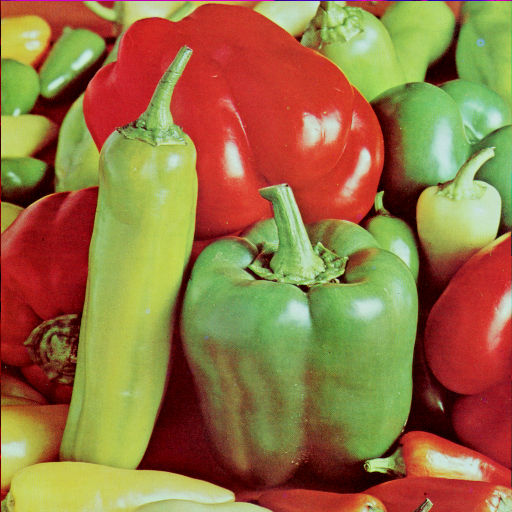
\includegraphics[width=0.5\textwidth]{preprocessing/peppers.png}
    \captionsource
    {A sample input image for the task of initial segmentation into superpixels}
    {A sample input image for the task of initial segmentation into superpixels}
    {Public-Domain Test Images for Homeworks and Projects \cite{peppers}}
     \label{fig:peppers}
\end{figure}
The chosen image has the size of $512px \times 512px$. For this sample image, the parameter defining the expected number of superpixels has been chosen to $300$. When it comes to compactness coefficient three values were chosen, 500, 50 and 2. First set of images shown in figure \ref{fig:peppers_mean_colour} presents one sample image divided into superpixels per one compactness coefficient value. A colour of each pixel in those images is the same as a mean colour of a superpixel which contains the given pixel.  
\begin{figure}[ht]
 \centering
  \begin{subfigure}[h]{0.32\textwidth}
    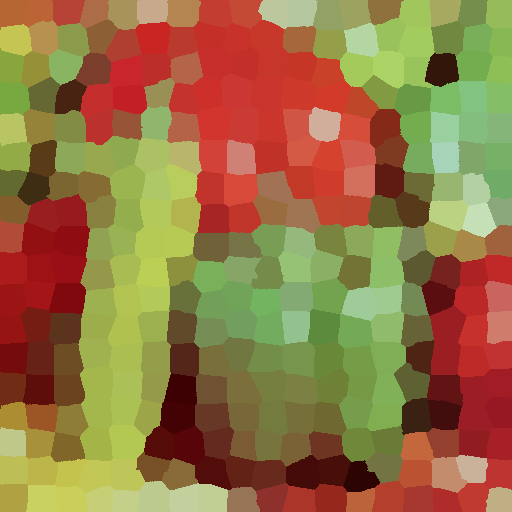
\includegraphics[width=\textwidth]{preprocessing/peppers_mean_300_500.png}
    \caption{Compactness 500}
    \label{fig:peppers_mean_colour_500}
  \end{subfigure}
  %
  \begin{subfigure}[h]{0.32\textwidth}
    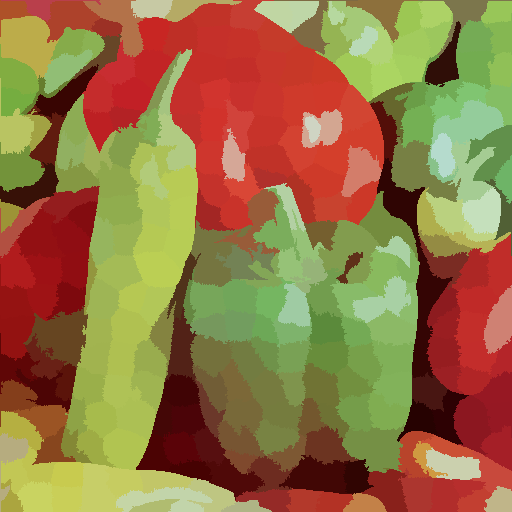
\includegraphics[width=\textwidth]{preprocessing/peppers_mean_300_50.png}
    \caption{Compactness 50}
    \label{fig:peppers_mean_colour_50}
  \end{subfigure}
  %
    \begin{subfigure}[h]{0.32\textwidth}
    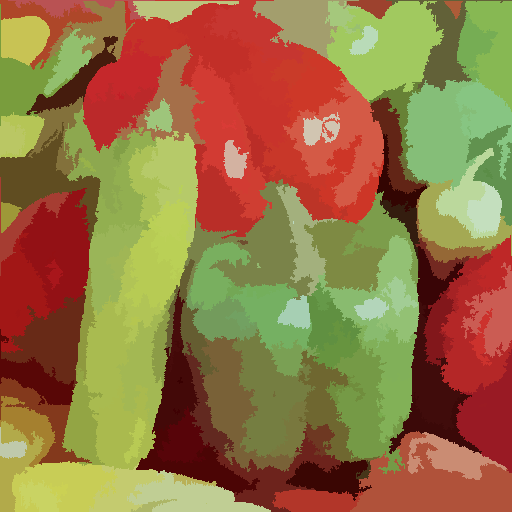
\includegraphics[width=\textwidth]{preprocessing/peppers_mean_300_2.png}
    \caption{Compactness 2}
    \label{fig:peppers_mean_colour_2}
  \end{subfigure}
    \caption{Division of a sample image into superpixels based on different values of compactness coefficient, with mean colour of each superpixel marked}%
    \label{fig:peppers_mean_colour}
\end{figure}
As visible, for large value of compactness coefficient being $500$ as shown in figure \ref{fig:peppers_mean_colour_500}, colours of the test image are blurred and it is hard to notice what this image presents without seeing it before the segmentation process. Segmented images with compactness coefficient for values $50$ and $2$ are quite similar.
Next set of images shown in figure \ref{fig:peppers_boundaries} present the results of the same processes of segmentation, however, this time superpixel borders are marked on the original image.
\begin{figure}[ht]
 \centering
  \begin{subfigure}[h]{0.32\textwidth}
    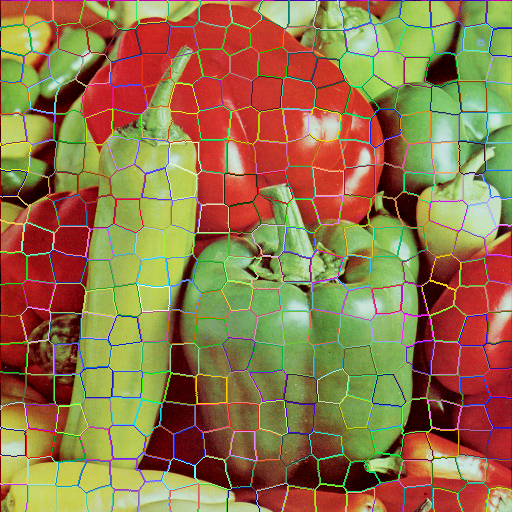
\includegraphics[width=\textwidth]{preprocessing/peppers_sp_border_300_500.png}
    \caption{Compactness 500}
    \label{fig:peppers_boundaries_500}
  \end{subfigure}
  %
  \begin{subfigure}[h]{0.32\textwidth}
    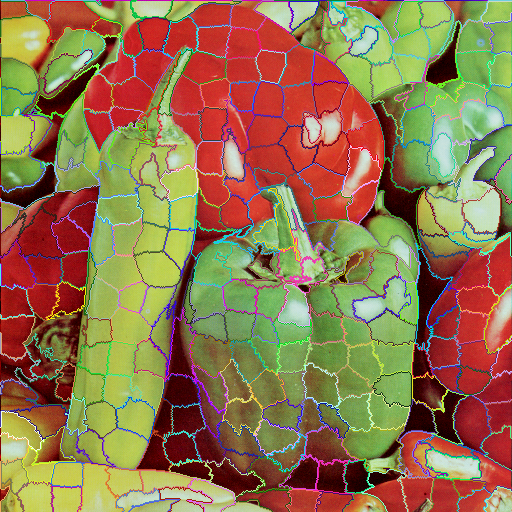
\includegraphics[width=\textwidth]{preprocessing/peppers_sp_border_300_50.png}
    \caption{Compactness 50}
    \label{fig:peppers_boundaries_50}
  \end{subfigure}
  %
    \begin{subfigure}[h]{0.32\textwidth}
    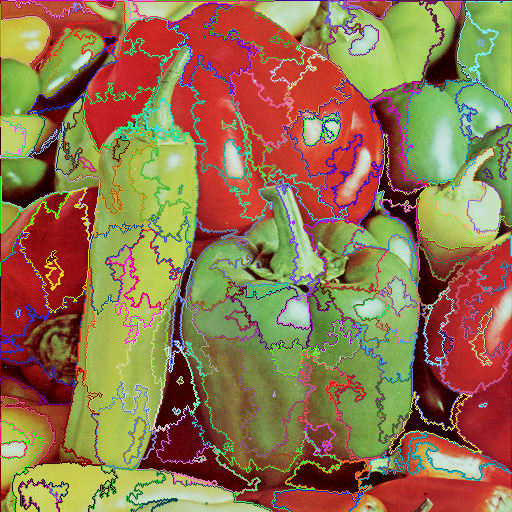
\includegraphics[width=\textwidth]{preprocessing/peppers_sp_border_300_2.png}
    \caption{Compactness 2}
    \label{fig:peppers_boundaries_2}
  \end{subfigure}
     \caption{Division of a sample image into superpixels based on different values of compactness coefficient, with borders of each superpixel marked}%
    \label{fig:peppers_boundaries}       
\end{figure}
As depicted in figure \ref{fig:peppers_boundaries_500} for large values of compactness coefficient the resulting superpixels have smooth boundaries and are roughly in the same size and square-like shape. A similar division is presented in figure \ref{fig:peppers_boundaries_50} for compactness coefficient of 50. Tough boundaries of of created superpixels are less smooth, still the size of them is pretty similar. Uniform size of superpixels is more suitable if an image is to be modelled with a graph, as they produce a regular lattice \cite{superpixels_compactness}, which is important for proper definition of superpixel neighbour that is required for computing of pairwise potentials. On the other hand, for small values of compactness coefficient, as in figure \ref{fig:peppers_boundaries_2}, the created superpixels adhere well to object boundaries, however, they differ largely in shape and size. Also the created lattice is highly irregular, as some objects are composed with only few superpixels, while in others even a small detail or a change of brightness is marked as a separate superpixel, which would make it difficult to assign this superpixel into a proper class.
Difference between shape of created superpixels is best visible on object boundaries. Figure \ref{fig:peppers_boundaries_zoom} depicts a zoomed view of superpixels that were created on the boundary between green and red peppers.
\begin{figure}[ht]
 \centering
  \begin{subfigure}[h]{0.32\textwidth}
    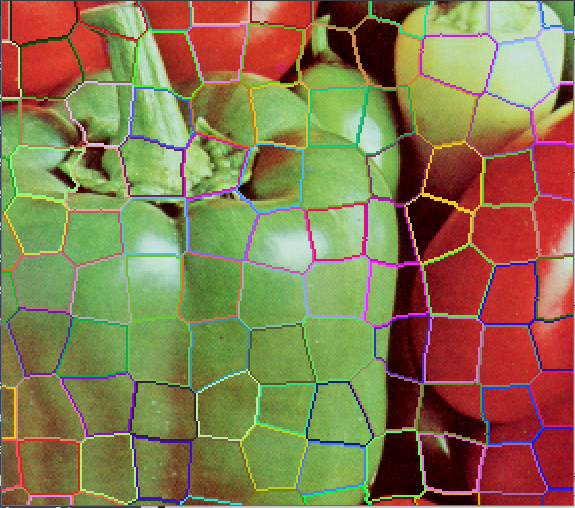
\includegraphics[width=\textwidth]{preprocessing/peppers_border_500.png}
    \caption{Compactness 500}
    \label{fig:peppers_boundaries_zoom_500}
  \end{subfigure}
  %
  \begin{subfigure}[h]{0.32\textwidth}
    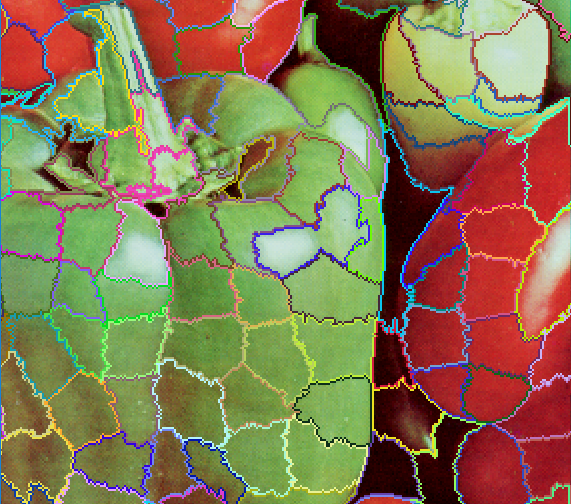
\includegraphics[width=\textwidth]{preprocessing/peppers_border_50.png}
    \caption{Compactness 50}
    \label{fig:peppers_boundaries_zoom_50}
  \end{subfigure}
  %
    \begin{subfigure}[h]{0.32\textwidth}
    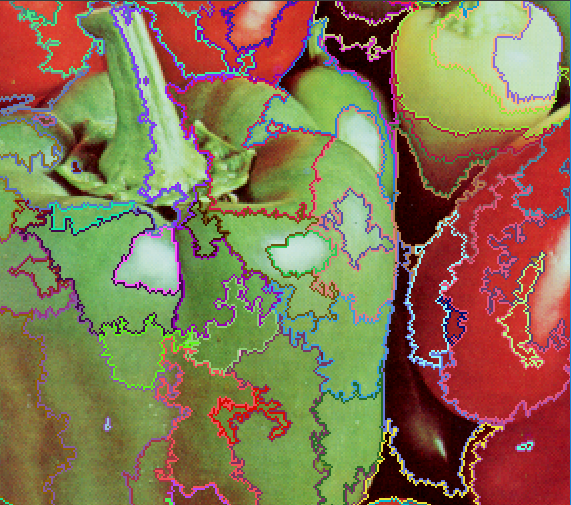
\includegraphics[width=\textwidth]{preprocessing/peppers_border_2.png}
    \caption{Compactness 2}
    \label{fig:peppers_boundaries_zoom_2}
  \end{subfigure}
     \caption{Division of a sample image into superpixels based on different values of compactness coefficient, with boundaries of each superpixel marked}%
    \label{fig:peppers_boundaries_zoom} 
\end{figure}
It is clear that for compactness coefficient of 500 the created superpixels do not comply with the already presented rule that no superpixel should be split by an object boundary. With such superpixel division semantic image segmentation would not be successful, as the information about object boundaries would be lost during the preprocessing stage. Hence, such a large value of this parameter does not give acceptable results. For compactness of 2, as shown in figure \ref{fig:peppers_boundaries_zoom_2}, created superpixels have totally different shapes. Furthermore, some superpixels are composed of only a really small number of pixels and they usually present artefacts of an image, which do not carry any important information for semantic segmentation and would only increase the computational complexity of this task. Therefore, too small values of compactness coefficient should also be avoided. Figure \ref{fig:peppers_boundaries_zoom_50} depicts superpixel segmentation that is the closest to optimal from all the presented divisions. The resulting superpixels properly define object boundaries at the same time creating a regular grid. What is more, small regions with changes of brightness that are irrelevant for semantic segmentation are not separated from surrounding pixels. Therefore, such division into superpixels would be applicable for further processing.

Thanks to the preprocessing stage, the number of inputs in the factor graph constructed upon a given image is largely lowered as instead of hundreds of thousands of pixels only few hundreds superpixels are needed. As a result the complexity of calculations and a required processing time are reduced. What is more, by division into superpixels pieces of image that are irrelevant for the task of semantic image segmentation are averaged and incorporated into one superpixel together with adjacent regions that carry more important information about the object they represent. This smoothing property is important for example for some slightly noised pixels or regions with the sudden change of brightness in few adjacent pixels.